% !Mode:: "TeX:UTF-8"
%%% Local Variables:
%%% mode: latex
%%% TeX-master: t
%%% End:

\chapter{面向对象的遥感影像的区间二型模糊聚类分割算法}
\label{cha:chap03}

\section{引言}
\label{sec:chap03-1}
由于遥感影像数据具有同物异谱、同谱异物等固有的不确定性,结合模糊数学理论对不确定信息刻画的优点,模糊C-均值聚类(Fuzzy c-means clustering, FCM)分割方法被广泛应用到遥感影像分析中 \cite{bezdek1984fcm}。同时,随着遥感影像空间分辨率的提高,高分影像数据具有更多的信息多样性和复杂性,遥感影像聚类方法由传统的基于像元发展为面向对象的聚类分割。本章内容从遥感影像特征信息表达和目标地物类别关系两个角度来表征遥感影像分类中的不确定性信息。首先设计了三角形模糊集值信息表达模型来表征影像分割单元信息,其次提出一种新的区间值度量方法计算两个三角形模糊集值数据的相异性,最后,改进了已有的二型模糊集合聚类分割方法来对影像数据建模,以刻画遥感影像数据的不确定性  \footnote{本章部分内容来自作者2018年发表于 SCI 期刊 \textit{Computers \& Geosciences} 上的文章 \cite{jiang2018enhanced}。 }。
%\footnote{注:本章部分内容来自本文作者2018年发表于《Computers \& Geosciences》 SCI期刊的文章} hh

\begin{figure}[!htb]
    \centering
    \includegraphics[width=0.9\textwidth]{compare_distribution}
    \caption{区间值相同但分布不同的数据比较}
    \label{fig:compare_distribution}
\end{figure}

\section{三角形模糊集值建模与相似性度量}
\label{sec:chap03-2}
当前,面向对象分割方法中对影像单元多采取均值数据建模 \cite{yu2012method} 和区间值数据建模 \cite{he2016remote} 。然而,这两种信息表达模型无法区分具有相同均值和区间值但内部分布不一致的分割单元。如图 \ref{fig:compare_distribution} 所示,每组模拟数据内的点集可以看作一个影像分割单元像素点集合,具有相同的均值和区间值的影像单元内像素点的分布差异明显。

模糊集(Fuzzy sets, FS) 是 Zadeh 教授 1965年提出的概念,通过建立适当的隶属度函数(Membership function, MF)来描述对象的不确定性 \cite{zadeh1965fuzzy}。 常见的隶属度函数有:三角形MF,梯形MF,截断高斯MF和钟形MF等。 FS 最常用和最基本的 MF 是三角形MF。 因此,文中利用三角形模糊集来定义三角形模糊集值数据模型。

\begin{definition}
    \label{define1}
    三角形模糊集值(Triangular Fuzzy Set Valued, TFSV)模型的定义
\end{definition}
三角形模糊集值数据由以下三个关键参数组成:$(a^-,0)$,$(a^m,1)$ 和 $(a^+,0)$。如图~\ref{fig:tfs} 所示,  几何上,$(a^-,0)$ 和 $(a^+,0)$ 组成三角形MF的下边缘;代数上,$(a^-,0)$ 和 $(a^+,0)$ 形成一个区间值,确保一定的变化范围。$(a^m,1)$是TFSV 数据的顶点,表征 FS 的最高置信度。
\begin{figure}[!htb]
    \centering
    \includegraphics[width=0.5\textwidth]{tfs}
    \caption{三角形模糊集 $\tilde{A}$ 示意图}
    \label{fig:tfs}
\end{figure}

聚类是根据某种相似性或距离将相似的对象聚为一类的无监督学习方法,相似性度量是聚类的核心要素。对于两个TFSV 数据$\tilde{A}$ 和 $\tilde{B}$,常见的相似性度量方法有以下几种:
\begin{enumerate}[(1)]
    \item 欧式距离(Euclidean distance)

          \begin{equation}
              \label{equ:eucliden}
              d_E(\tilde{A}, \tilde{B}) = \sqrt{\sum_{x \in X} |\tilde{A}(x)-\tilde{B}(x)|^2 }, x \in X
          \end{equation}
          $\tilde{A}$ 和 $\tilde{B}$ 的欧式距离 $d_E(\tilde{A}, \tilde{B})$ 被看作是集合对应元素差值平方和的平方根。
    \item 城市距离(City-block distance)

          \begin{equation}
              \label{equ:cityblock}
              d_C(\tilde{A}, \tilde{B}) = \sum_{x \in X}|\tilde{A}(x)-\tilde{B}(x)| , x \in X
          \end{equation}
          $\tilde{A}$ 和 $\tilde{B}$ 的城市距离 $d_C(\tilde{A}, \tilde{B})$ 被看作是集合对应元素差值绝对值的和。
          %  \item 切比雪夫距离(Tchebyshev distance)

          %        \begin{equation}
          %            \label{equ:tchebyshev}
          %            d_T(\tilde{A}, \tilde{B}) = \sqrt[\infty]{\int_X |\tilde{A}(x)-\tilde{B}(x)|^\infty dx }, x \in X
          %        \end{equation}
          %        $\tilde{A}$ 和 $\tilde{B}$ 的切比雪夫距离 $d_T(\tilde{A}, \tilde{B})$ 被看作是集合对应元素差值积分的一个极限值。
    \item 豪斯多夫距离(Hausdorff distance)

          豪斯多夫距离最开始为区间或普通集合设计,两个普通集合 $A$ 与 $B$ 的豪斯多夫距离为:
          \begin{equation} \label{eq:haus1}
              d_H(A, B) = \max \Big  \lbrace \sup_{a \in A} \inf_{b \in B} \abs{a-b}, \sup_{b \in B} \inf_{a \in A} \abs{a-b} \Big  \rbrace
          \end{equation}
          将其推广到模糊集,可以考虑模糊集 $\tilde{A}$ 和 $\tilde{B}$的一个 $\alpha-cut$ 截集  \cite{zadeh1965fuzzy} $d_H^{\alpha} (\tilde{A}, \tilde{B})$,则有:
          \begin{equation}\label{eq:haus_alpha}
              \begin{split}
                  d_H^{\alpha} (\tilde{A}, \tilde{B}) = \max \Big \lbrace \sup_{a \in \tilde{A_{\alpha}}} \inf_{b \in \tilde{B_{\alpha}}} \abs{a-b}, \sup_{b \in \tilde{B_{\alpha}}} \inf_{a \in \tilde{A_{\alpha}}}
                  \abs{a-b} \Big \rbrace
              \end{split}
          \end{equation}
          其中,$\inf$ 和 $\sup$ 分别表示取集合的最大下界和最小上界。模糊集是度量空间的非空紧致和有限子集,所以等式~\ref{eq:haus_alpha} 中的 $\inf$ 和 $\sup$ 操作可分别替换为 $\min$ 和 $\max$ 操作, 即
          \begin{equation}\label{eq:haus_alpha2}
              \begin{split}
                  d_H^{\alpha} (\tilde{A}, \tilde{B}) = \max \Big \lbrace \max_{a \in \tilde{A_{\alpha}}} \min_{b \in \tilde{B_{\alpha}}} \abs{a-b}, \max_{b \in \tilde{B_{\alpha}}} \min_{a \in \tilde{A_{\alpha}}} \abs{a-b} \Big \rbrace
              \end{split}
          \end{equation}
          然后对 $\tilde{A}$ 和 $\tilde{B}$ 所有可能的$\alpha-cut$ 截集积分,就可得到模糊集 $\tilde{A}$ 和 $\tilde{B}$的豪斯多夫距离:
          \begin{equation}\label{eq:haus2}
              \begin{split}
                  d_H(\tilde{A}, \tilde{B}) = \int_0 ^1 d_H^{\alpha} (\tilde{A}, \tilde{B}) d \alpha = \int_0 ^1 \max \Big \lbrace \max_{a \in \tilde{A_{\alpha}}} \min_{b \in \tilde{B_{\alpha}}} \abs{a-b}, \max_{b \in \tilde{B_{\alpha}}} \min_{a \in \tilde{A_{\alpha}}} \abs{a-b} \Big \rbrace  d \alpha
              \end{split}
          \end{equation}

\end{enumerate}



那么,如何选择合适的距离来度量两个模糊集的相似性呢?对于模糊集 $\tilde{A}$ 和 $\tilde{B}$,如图~\ref{fig:set_location} 所示,我们考虑在同一坐标系内, $\tilde{A}$ 和 $\tilde{B}$ 只存在三种位置关系:相交、包含和不相交。

\begin{figure}[!htb]
    \centering
    \includegraphics[width=0.9\textwidth]{set_location}
    \caption{$\tilde{A}$ 和 $\tilde{B}$ 位置关系示意图。 (a)相交; (b)$\tilde{A}$ 包含集合$\tilde{B}$;  (c)不相交.}
    \label{fig:set_location}
\end{figure}

为了比较各种位置关系下两个模糊集间上述各种距离的大小关系。文中设计以下实验:如图~\ref{fig:distance_compare}(a) 所示,$\tilde{B}$ 固定不动,将$\tilde{A}$ 沿$\textbf{X}$ 轴从左向右移动,分别计算各相对位置下$\tilde{A}$ 和$\tilde{B}$ 对应位置的距离。结果如图~\ref{fig:distance_compare}(b) 所示(图中$0-cut$ 和$1-cut$ 截集的豪斯多夫距离后面会讨论),$\tilde{A}$ 位于$(a,b)$ 区间内时,$\tilde{A}$ 和$\tilde{B}$ 相交,以上四种距离均可度量$\tilde{A}$ 和$\tilde{B}$ 的相似性。 然而,在两者不相交时(图中$\tilde{A}$ 位于$(-\infty, a)$ 和$(b,+\infty)$ 区间内)无论$\tilde{A}$ 和$\tilde{B}$ 相距多远,欧式距离和城市距离均为一固定常量,只有豪斯多夫距离可以精确度量上述三种位置下两个模糊集的相似性。

\begin{figure}[!htb]
    \centering
    \includegraphics[width=0.9\textwidth]{distance_compare}
    \caption{不同位置下,$\tilde{A}$ 和 $\tilde{B}$ 两者间各种距离比较图。}
    \label{fig:distance_compare}
\end{figure}

然而,计算两个模糊集之间的豪斯多夫距离具有较高的计算复杂度,导致其在模糊聚类迭代更新中难以适用。另外,Zadeh 教授在可能性分布理论\cite{zadeh1978fuzzy} 中提到: 模糊集作为一个弹性约束值, 若使用区间距离度量, 而不是一个单一固定值来度量两个模糊集间相似性可以获取产生更高的识别能力。因此, 文中尝试引入一种新的基于豪斯多夫距离的区间距离度量方法来度量三角形模糊集的相似性。

首先,考虑模糊集合的特性, 文献 \cite{zadeh1978fuzzy} 中定义了模糊集的$\alpha-cut$ 截集并提出了模糊集的$\alpha-cut$ 截集表现定理,其中提到任何模糊集都可以由它指定的$\alpha-cut$ 截集来表示。在所有的截集中,有两个截集是最重要与最具有代表性的,它们就是$0-cut$ 和$1-cut$ 截集,分别代表模糊集和的支撑集和置信集合。模糊集$\tilde{A}$ 的支持集$0-cut$ 包含$\tilde{A}$ 中非零的所有元素,体现了模糊集的可能性;而$\tilde{A}$ 的置信集$1-cut$ 包含元素的隶属度均为$1$,这表明$1-cut$ 截集中所有元素都有最高的隶属度和置信度,体现了模糊集的必要性。此外,最近一些关于$\alpha-cut$ 截集的研究对任一模糊集,仅使用$0-cut$ 和$1-cut$ 截集就可近似拟合模糊集的质心;此外,任意其他$\alpha -cut$ 截集$ (0 \leq \alpha \leq 1)$ 都可以表示为$0-cut$ 和$1-cut$ 截集的广义线性组合\cite{liu2008efficient}。

根据公式\ref{eq:haus_alpha2}, 我们分别可以获得$\tilde{A}$ 和$\tilde{B}$ 的$0-cut$ 和$1-cut$ 的豪斯多夫距离为$d_H^{0} (\tilde{A}, \tilde{B})$ 和 $d_H^{1} (\tilde{A}, \tilde{B})$。基于上面提到的可能性分布理论和模糊集的$\alpha-cut$ 截集表现定理,我们可以定义两个三角形模糊集间$\tilde{A}$ 和$\tilde{B}$ 间一种新的区间值距离$d_I (\tilde{A}, \tilde{B})$ 为下式:
\begin{equation}\label{eq:interval}
    \begin{split}
        d _{I} (\tilde{A},\tilde{B}) = [\min \lbrace d_0 (\tilde{A},\tilde{B}),d_1(\tilde{A},\tilde{B}) \rbrace, \max \lbrace d_0(\tilde{A},\tilde{B}), d_1 (\tilde{A},\tilde{B}) \rbrace ]
    \end{split}
\end{equation}
图~\ref{fig:distance_compare} 中的结果($0-cut$ 和$1-cut$)也表明$d _{I} (\tilde{A},\tilde{B})$ 能够度量两个模糊集不相交时的相似性;另外,还可以看出文中新定义的距离$ d _{I} (\tilde{A},\tilde{B})$ 是$ d _{H} (\tilde{A},\tilde{B})$的弹性膨胀,即有:
\begin{equation}\label{eq:expand_in}
    \begin{split}
        d _{H} (\tilde{A},\tilde{B}) \in d _{I} (\tilde{A},\tilde{B})
    \end{split}
\end{equation}
公式~\ref{eq:expand_in}的证明步骤由于篇幅过大,可参考本文作者已发表文章\cite{jiang2018enhanced} 的附录一。

一个相似性度量能够定位为距离,当且仅当其能满足距离度量三个条件,即非负性、对称性和三角不等式。假定$\tilde{A}$、$\tilde{B}$ 和$\tilde{C}$是任意三个三角形模糊集,则需要满足以下特性:
\begin{enumerate}[(1)]
    \item \textsl{非负性}: $d_I(\tilde{A}, \tilde{A}) = 0$
    \item\textsl{对称性}: $d_I(\tilde{A}, \tilde{B}) = d_I(\tilde{B}, \tilde{A})$
    \item  \textsl{三角不等式}: $d_I(\tilde{A}, \tilde{C}) \leq d_I(\tilde{A}, \tilde{B}) + d_I(\tilde{B}, \tilde{C})$
\end{enumerate}
证明过程较复杂,可参考本文作者已发表文章\cite{jiang2018enhanced} 的附录二。

综上所述,本节针对面向对象分割单元定义了TFSV 数据模型,同时,结合模糊集与可能性分布定理特性,针对新提出的TFSV 数据类型,本文新提出了一种区间值的距离度量方法,来度量两个TFSV 数据间的相似性。


\section{面向对象的改进型区间二型模糊遥感影像聚类方法}
\label{sec::chap03-3}


\subsection{算法整体框架}
\label{subsec::chap03-3}
本章提出基于三角形模糊集值的区间二型模糊聚类方法(Triangular Fuzzy Set Valued Interval Type 2 Fuzzy Clustering Method, TFSV-IT2FCM)主要用于提高高分辨率遥感影像无监督聚类分割精度。图~\ref{fig:framework} 展示了该面向对象分类方法的总体处理流程,具体可分为以下几点:

\begin{enumerate}[Step 1:]
    \item 影像分割与对分割单元的TFSV 数据建模

          高分影像被分割为具有同质性的像素单元集合.对分割单元提取特征,并构建 TFSV 模型;
    \item 模糊聚类分析

          使用TFSV-IT2FCM 算法对高分影像分割单元的TFSV 模型数据聚类,IT2FCM 算法的距离度量使用文中新提出的区间距离$d_I$;
    \item 聚类结果的后处理

          使用类别组合方法对聚类分割的结果处理,得到高分影像最终得分割结果。
\end{enumerate}

\begin{figure}[!htb]
    \centering
    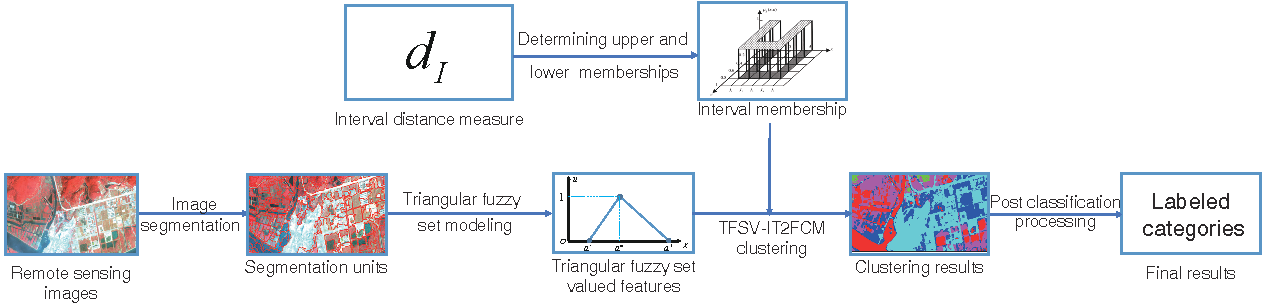
\includegraphics[width=1.0\textwidth]{framework}
    \caption{面向对象的改进型区间二型模糊遥感影像聚类算法框架图}
    \label{fig:framework}
\end{figure}


\subsection{面向对象的TFSV 模型}
\label{subsec::chap03-3-1}

\subsubsection{影像分割}
\label{subsec::chap03-3-1-1}

目前,遥感影像常用的像元分割算法包含基于分水岭的算法,基于直方图的方法和聚类方法等\cite{roerdink2000watershed}。简单线性迭代聚类(SLIC)算法具有高计算效率和可选数量的分段单元\cite{achanta2012slic},因此本章使用SLIC 超像素分割算法提取遥感影像的分割单元。 SLIC 算法的关键步骤如下:
\begin{enumerate}[(I)]
    \item 计算遥感影像梯度获取影像梯度图;
    \item 初始化梯度图中的聚类中心;
    \item 将遥感影像从SPOT5 格式转换为CIELAB 颜色空间计算像元间的相似度;
    \item 使用SLIC 算法对CIELAB 彩色图像进行分割,以获得影像同质性分割单元。
\end{enumerate}

对高分影像$\bm{I}$ ,使用SLIC 分割算法获得影像分割单元 $\bm{SS}$,为:
\begin{equation}\label{eq:image_ss}
    \begin{split}
        \bm{SS} = \lbrace \bm{B_1}, \bm{B_2},\bm{\cdots}, \bm{B_n} \rbrace
    \end{split}
\end{equation}
其中$\bm{B_i}(1 \leq i \leq n)$ 表示第$i$ 个分割单元,$n$ 表示分割单元的总数。 $\bm{B_i}(i=1,2,\cdots, n)$ 是一个$j \times p$ 矩阵,其中$j$ 表示每个波段包含的像素数目,$p$ 表示图像通道数。


\subsubsection{影像单元的TFSV 数据建模}
尽管文献\cite{he2016remote} 中已经证明:对于影像分割单元,区间值的特征比均值特征更有效,但是影像分割单元的不确定性不能被充分的表达。因此,文中使用定义 \ref{define1} 的TFSV 数据模型$\bm{\tilde{A_i}}$  来提取影像单元$\bm{B_i}$ 的特征:
\begin{enumerate}[ 1)]
    \item 基于影像分割单元$\bm{B_i}$内像素的均值和方差特性,可以获得一个$p$ 维的区间值向量,记为$\bm{X_i}$,如下:
          \begin{equation}\label{eq:eq-1}
              \bm{X_i} = [\bm{X_{i}^{down}},\bm{X_i^{up} }] = [\max{\lbrace 0,\bm{\mu_i} - \alpha \times \bm{\sigma_i} \rbrace}, \bm{\mu_i} + \alpha \times \bm{\sigma_i}]
          \end{equation}

          其中$\bm{\mu_i} = [\mu_{1}, \mu_2,\cdots,\mu_p]^T$,$\bm{\sigma_i} = [\sigma_{1},\sigma_2,\cdots,\sigma_p] ^T$ 是第$i$个分割单元$\bm{B_i}$ 的均值和方差,$\alpha$ 是控制区间值大小的超参数,$p$ 是遥感影像的波段数。
    \item 分割单元是邻近同质像素点的集合,基于统计学特性,等式\ref{eq:eq-1} 中的向量$\bm{X_i} = [\bm{X_{i}^{down}},\bm{X_i^{up} }]$ 除了少数异常点外包含分割单元$\bm{B_i}$中的绝大部分点。因此,从$\bm{X_i}$ 中导出参数 $(\bm{X_{i}^{down}},0)$ 和$(\bm{X_i^{up}},0)$来构造$\bm{\tilde{A_i}}$ 的底边。
    \item $\bm{\tilde{A_i}}$ 的顶点由$(\bm{med_i},1)$ 组成。因中值不受极值的影响,并且对噪声点和异常值具有很高的鲁棒性,这里$\bm{med_i}$ 取$\bm{B_i}$ 的中值。
\end{enumerate}


类似地,影像的每个分割单元都可以被表征为一个 TFSV 数据模型,分割单元的集合$\bm{SS} = \lbrace \bm{B_1}, \bm{B_2},\bm{\cdots}, \bm{B_n} \rbrace$ 可以被表示为:

\begin{equation}\label{eq:eq-2}
    \bm{SS} \to \lbrace \bm{\tilde{A_1}}, \bm{\tilde{A_2}},\bm{\cdots}, \bm{\tilde{A_n}} \rbrace
\end{equation}

其中$\bm{SS}$ 是一个$n \times p$ 矩阵,$\bm{\tilde{A_i}}$ 是$\bm{B_i}$ 对应的$p$ 维TFSV 数据,$n$ 表示分割单元的数目。


\subsection{基于TFSV 数据模型的面向对象模糊聚类方法}
\label{subsec::chap03-3-2}


\subsubsection{区间二型模糊隶属度}
\label{subsec::chap03-3-3-2-1}
区间二型模糊聚类算法(Interval type 2 fuzzy clustering method, IT2FCM) 使用一个区间值来表示隶属度值。文献\cite{hwang2007uncertain} 中使用两个模糊化指数$m_1$ 和$m_2$ 得到区间二型隶属度函数(Interval type 2 membership function,IT2MF) 的上界和下界,从而将一型模糊集(Type 1 fuzzy sets, T1FS) 扩展为二型模糊集(Type 2 fuzzy sets, T2FS)。然而,IT2FCM 算法对模糊指数$m_1$ 和$m_2$ 的取值敏感。与传统FCM 算法相比,不恰当的$m_1$ 和$m_2$ 取值会导致更差的实验结果。因此,基于公式~\ref{eq:interval} 中新定义的区间值距离度量,类似FCM 算法,本文仅使用一个模糊指数$m$ 来表达IT2MF。


假定样本$\bm{\tilde{X}} = (\tilde{X_1}, \tilde{X_2},\cdots, \tilde{X_p})^T$ 和聚类中心$\bm{\tilde{V}} = (\tilde{V_1}, \tilde{V_2},\cdots, \tilde{V_p})^T$ 是两个形如公式~\ref{eq:eq-2} 的$p$ 维TFSV 数据,其中$\tilde{X_i}$ $(1 \leq i \leq p)$ 是一个一维TFSV,由$(X_{i}^{down}, 0)$,$(X_{i}^{up}, 0)$和$(X_i^{med}, 1)$ 这三个参数构成;类似地,$\tilde{V_i}$ 由$(V_{i}^{down}, 0)$,$(V_{i}^{up}, 0)$ 和$(V_i^{med}, 1)$三个参数组成。$\tilde{X_i}$ 和$\tilde{V_i}$ 的$0-cut$ 和$1-cut$ 豪斯多夫距离分别为:

\begin{equation}\label{eq:eq-3}
    \begin{split}
        d_0 (\tilde{X_i}, \tilde{Y_{i}}) = \max \Big \lbrace \abs{X_i^{down} - Y_i^{down}}, \abs{X_i^{up} - Y_i^{up}} \Big \rbrace
    \end{split}
\end{equation}
和
\begin{equation}\label{eq:eq-4}
    \begin{split}
        d_1 (\tilde{X_i}, \tilde{V_{i}}) = \Big\lbrace |X_i^{med} - V_i^{med}| \Big\rbrace
    \end{split}
\end{equation}
$\tilde{X_i}$ 和$\tilde{V_{i}}$ 的区间值距离$d_{I} (\tilde{X_i}, \tilde{V_i})$ 即为:
\begin{equation}\label{eq:eq-5}
    \begin{split}
        d_{I} (\tilde{X_i}, \tilde{V_i}) = [\min \lbrace d_0 (\tilde{X_i}, \tilde{V_{i}}) , d_1 (\tilde{X_i}, \tilde{V_{i}}  \rbrace,\max  \lbrace d_0 (\tilde{X_i}, \tilde{V_{i}}) , d_1 (\tilde{X_i}, \tilde{V_{i}}  \rbrace]
    \end{split}
\end{equation}
从而,$\bm{\tilde{X}}$ 和$\bm{\tilde{V}}$ 间的区间值距离$d_{I} (\bm{\tilde{X}}, \bm{\tilde{V}})$ 可以被表示为:

\begin{equation}\label{eq:eq-6}
    \begin{split}
        d_{I} (\bm{\tilde{X}}, \bm{\tilde{V}}) = \max \lbrace d_{I} (\tilde{X_i}, \tilde{V_i}) \rbrace, i =1.2.\cdots,p
    \end{split}
\end{equation}

与FCM 算法类似,新提出的面向对象的TFSV-IT2FCM 算法求解需要最小化以下目标函数:

\begin{equation}\label{eq:eq-7}
    J(\bm{U};\bm{V}) = \sum _{j=1} ^{n} \sum_{i=1} ^K (U_{ij})^m d^2(X_i,V_j)
\end{equation}
其中$m (m>1)$ 是模糊指数,$d^2(X_i,V_j) = d_{I} (\tilde{X_i}, \tilde{V_j})$ 是依据公式~\ref{eq:interval} 定义的样本$X_i$ 和$V_j$ 间的区间值距离。为了最小化目标函数$J$,有:

\begin{equation}\label{eq:12}
    \begin{split}
        U_{ij} = \frac{1}{\sum_{k=1}^K {(\frac{d_{ji}}{d_{ki}})}^{\frac{2}{m-1}}}
    \end{split}
\end{equation}

在TFSV-IT2FCM 算法中,模糊指数$m$ 的上界和下界以及区间值$d^2(X_i,V_j)$ 用来描述不确定性。区间隶属度的上界$\overline{u}_{ij}$ 和下界$\underline{u}_{ij}$ 分别为:

\begin{equation}\label{eq:13}
    \begin{split}
        \overline{u}_{ij} = \max \Bigg \lbrace \frac{1}{\sum_{k=1}^K {(\frac{d_{ji}^0}{d_{ki}^0})}^{\frac{2}{m-1}}}, \frac{1}{\sum_{k=1}^K {(\frac{d_{ji}^1}{d_{ki}^1})}^{\frac{2}{m-1}}} \Bigg \rbrace
    \end{split}
\end{equation}
和
\begin{equation}\label{eq:14}
    \begin{split}
        \underline{u}_{ij} = \min \Bigg \lbrace \frac{1}{\sum_{k=1}^K {(\frac{d_{ji}^0}{d_{ki}^0})}^{\frac{2}{m-1}}}, \frac{1}{\sum_{k=1}^K {(\frac{d_{ji}^1}{d_{ki}^1})}^{\frac{2}{m-1}}} \Bigg \rbrace
    \end{split}
\end{equation}
其中$d_{ji}^0$ 和$d_{ji}^1$ 分别是$\tilde{X_i}$ 和$\tilde{V_j}$ 的$0-cut$ 距离和$1-cut$ 距离度量,由区间值距离$d_{I} (\tilde{X_i}, \tilde{V_j})$ 计算得出。


\subsubsection{TFSV-IT2FCM 算法}
\label{subsubsec::chap03-3-3-2-2}
与FCM 算法不同,文中提出的TFSV-IT2FCM 算法核心是一个IT2FS,无法直接通过降型去模糊化,需要先计算IT2FS 的质心将IT2FS 转换为T1FS,再去模糊化得到明确集\cite{karnik2001centroid}。 文中使用EKM 降型算法\cite{wu2009enhanced} 降型和去模糊化,从而获取精确的聚类中心。降型后的聚类中心点可表示为

\begin{equation}\label{eq:17}
    \begin{split}
        \bm{V_j} = [\bm{V_j^L}, \bm{V_j^R}]
    \end{split}
\end{equation}
通过去模糊化后得到的明确集聚类中心为:

\begin{equation}\label{eq:18}
    \begin{split}
        \bm{V_j} = \frac{\bm{V_j^L}+\bm{V_j^R}}{2}
    \end{split}
\end{equation}

\begin{figure}[H]
    \centering
    \includegraphics[width=0.8\textwidth]{tfsvit2}
    \caption{TFSV-IT2FCM 算法流程图}
    \label{fig:tfsvit2}
\end{figure}

整个TFSV-IT2FCM 算法框架如图~\ref{fig:tfsvit2} 所示, 算法的详细描述如下:
\begin{enumerate}[(1)]
    \item 初始化

          初始化实验聚类参数个数$K (2 \leq K \leq N)$,在实验$1$、$2$、$3$ 中分别设置$K=5$、$5$ 和$6$。 初始化模糊指数$m = 2.0 \; (1 < m < \infty)$ , 迭代阈值$\varepsilon = 0.0001 \;(\varepsilon > 0)$,最大迭代次数$T = 500$,初始 $t = 1$,初始化区间膨胀参数$\alpha = 0.8$。其中超参数$m$ 和$\alpha$ 依赖具体的问题和实验数据。在本实验中, 当$m = 2.0$ 和$\alpha = 0.8$能取得最优实验效果。

    \item TFSV 数据建模

          使用SLIC 算法获取影像的分割单元$\bm{SS} = \lbrace \bm{B_1}, \bm{B_2},\bm{\cdots}, \bm{B_n} \rbrace$ ,然后转化为TFSV 类型数据$\lbrace \bm{\tilde{X_1}},\bm{\tilde{X_2}},\cdots, \bm{\tilde{X_n}}  \rbrace$ 作为训练样本。初始化TFSV 的聚类中心$\bm{\tilde{V}} = \lbrace \bm{\tilde{V_1}}, \bm{\tilde{V_2}}, \cdots, \bm{\tilde{V_K}} \rbrace$为 $\bm{\tilde{V^0}}$,其中$\bm{\tilde{V_k^0}},(1 \leq k \leq K)$ 由参数$(v_k^l, 0)$、$(v_k^r, 0)$ 和$(v_k^{mid}, 1)$构成。

    \item 聚类迭代更新

          在TFSV-IT2FCM 算法迭代中得到模糊划分矩阵$\bm{U} = [U_{ij}]_{n \times K}$,其中 $U_{ij} = [ \underline{u}_{ij}, \overline{u}_{ij}]$ 如公式\ref{eq:13} 和\ref{eq:14} 所示。聚类中心$[\tilde{v_l},\tilde{v_r}]$ 由EKM 算法降型获取。然后,将降型后的聚类中心去模糊化,得到明确集的聚类中心为
          \begin{equation}\label{eq:19}
              \tilde{v} = \frac{\tilde{v_l}+ \tilde{v_r}}{2}
          \end{equation}

    \item 迭代中止

          如果迭代过程满足 $||\bm{\tilde{V}^t} - \bm{\tilde{V}^{t+1}}|| \leq \varepsilon$ 或$t \geq T$ 即停止迭代; 否则,令$t = t+1$ 并跳到步骤 (3) 。距离$||\bm{\tilde{V}^t} - \bm{\tilde{V}^{t+1}}||$ 可由$d_I(\bm{\tilde{V}^t},\bm{\tilde{V}^{t+1}})$ 取均值得到,即
          \begin{equation}\label{eq:20}
              ||\bm{\tilde{V}^t} - \bm{\tilde{V}^{t+1}}|| = \frac{d_0(\bm{\tilde{V}^t}, \bm{\tilde{V}^{t+1}})+ d_1(\bm{\tilde{V}^t}, \bm{\tilde{V}^{t+1}})}{2}
          \end{equation}

    \item 硬划分

          区间二型的模糊划分矩阵$\bm{U} = [U_{ij}]_{n \times K}$ 可以降型为
          \begin{equation}\label{eq:21}
              U_{ij} = \frac{\underline{u}_{ij} + \overline{u}_{ij}}{2}
          \end{equation}
          其中 $U_{ij} = [\underline{u}_{ij}, \overline{u}_{ij}]$。然后,求出$\bm{\tilde{X}_i}$ 到聚类中心$\bm{\tilde{V}_k}$ 的最大隶属度$U_{ik}$ ,其中$k = 1, 2,\cdots, K$。根据最大隶属度原则,将$\bm{\tilde{X}_i}$ 划分到类别$\bm{\tilde{V}_k}$ 。



\end{enumerate}


\subsection{后处理}
\label{subsec::chap03-3-3}

经过像元分割与非监督模糊聚类,可以得到遥感影像的初始分类结果。使用CORINE 地物覆被处理系统\footnote{CORINE (Coordination of Information on the Environment) 是欧洲委员会于1985年提出的环境信息协调系统,其包含44个类别的地物覆被,常用于地物覆被的后处理。官方网址:\url{https://land.copernicus.eu/pan-european/corine-land-cover}.} 对初始聚类结果进行人工类别合并,实现基于高分影像识别的高级地物覆被分类\cite{zhang2011progress}。

\section{实验结果}
\label{sec::chap03-4}
本章新提出的面向

\section{本章小结}
\label{sec::chap03-5}
总结 balabala..
